\chapter{Methodology}\label{Methodology}
In this chapter the data mining methods used to retrieve movement patterns from the TU Delft eduroam Wi-Fi log data will be described in detail. \autoref{figure:workflow} gives an overview of the main workflow to derive movement patterns from the Wi-Fi log. First the raw Wi-Fi log is preprocessed to get states at two different spatial levels (building- and building-part level). A state is defined as a time interval during which a particular device is located in a certain area. An example of a state on building level is: device A is located at Library from 11:00 to 12:00. An example on building part level is: device A is located at canteen from 11:00 to 12:00. In the pre-processing phase the data is enriched with 'world' states, reduced by grouping states and cleaned by filtering out 5 minute states representing people that only pass by a building without actually entering it. The insertion of world states enables the detection of movement from and to the campus in the case of building level, and movement from and to the building in the case of building-part level. The states resulting from the pre-processing are used to retrieve movements at both spatial levels. A movement is defined by the change from one state to the next subsequent state, where the different states must be at a different locations. Furthermore, the building level states are used to retrieve trajectories for each device. A trajectory is defined as an ordered list of states. The trajectory thus stores the entire route or trajectory the particular person travelled. For the building-part level no trajectories are retrieved. For building-part level a graph is made for BK-city. In these graph the nodes represent the different building-part and the edge follow movement space, such as corridors and stairs. Using the shortest path in the graph, the route of the movements within BK-city can be visualized in more detail. For building level no graph is created and both trajectories and movements are visualized simply as a straight line. In addition to the maps at both the building and building-part spatial level, movement time series are created for both spatial levels. Together these maps and time series are used to identify different types of movement patterns. 
\\
\begin{figure}[H]
\centering
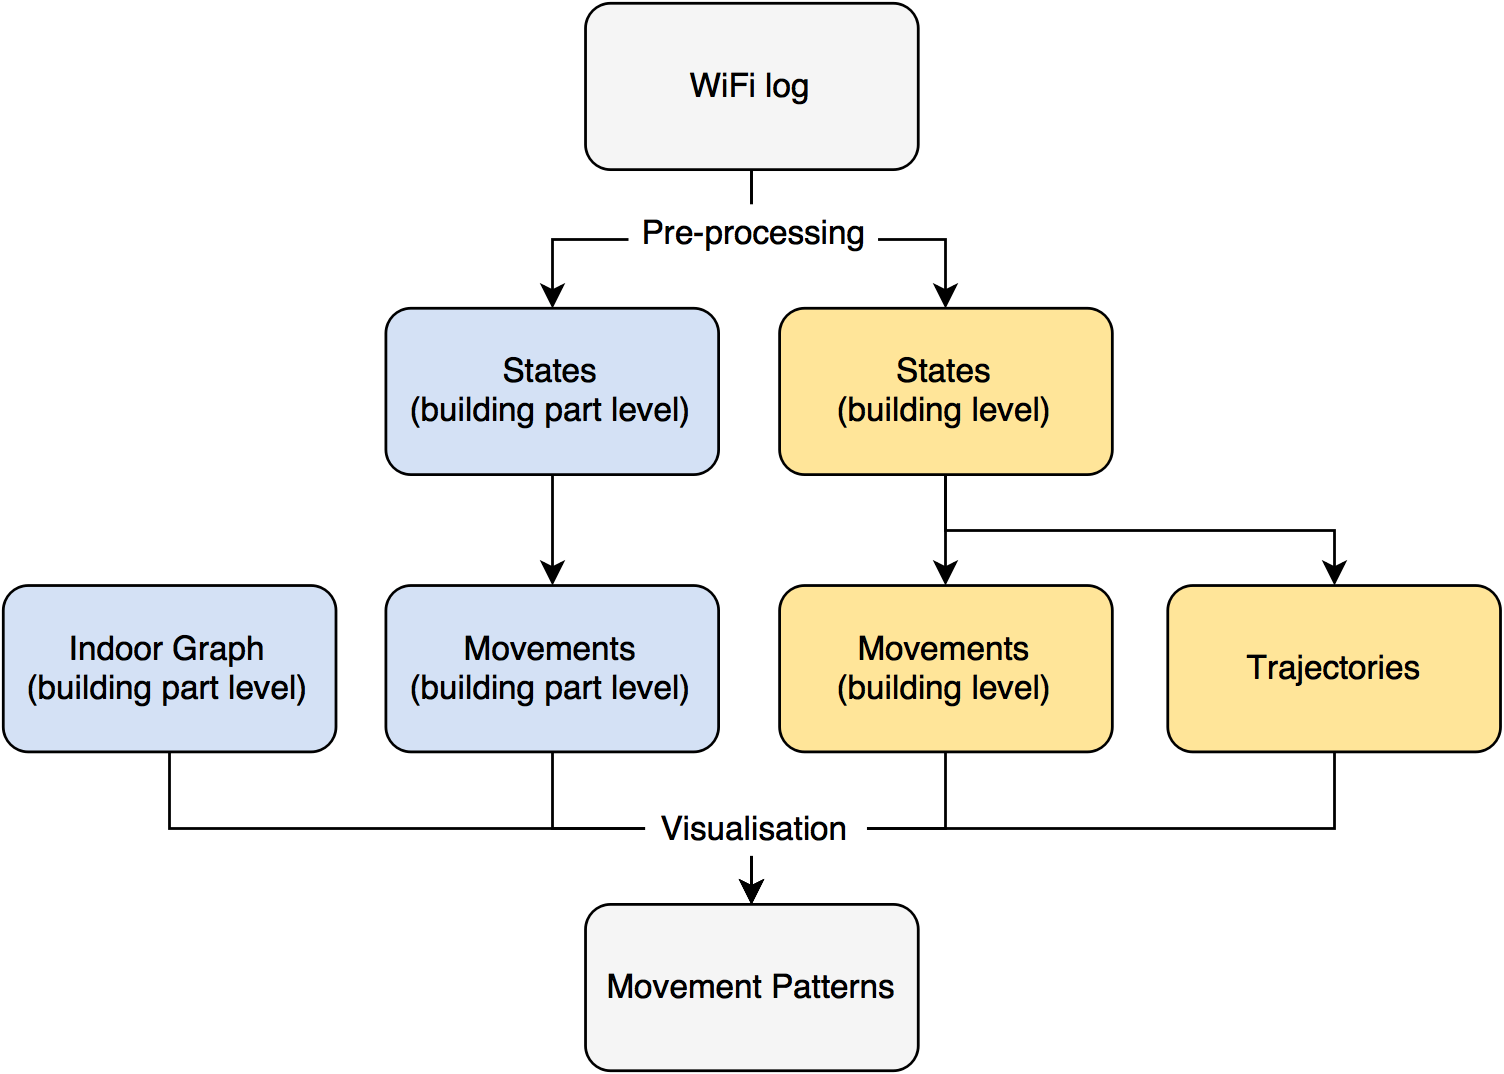
\includegraphics[scale=0.25]{methodology_workflow}
\captionsetup{justification=centering}
\caption{Grouping}
\label{figure:workflow}
\end{figure}
In the following three chapter all these steps to derive different movement patterns will described in more detail. First \autoref{preprocessing} describes the various pre-processing steps to clean, reduce and enrich the raw data. Subsequently \autoref{movement} addresses the creation and visualization of movement on building level, this includes movement between buildings and movement from and to the campus. \autoref{trajectories} covers the creation and visualization of trajectories on building level. Finally \autoref{indoormovement} discusses the creation of the graph and movements for BK-city (building-part level) and visualization of these movements. The latter three of these chapters also show several results. The focus of this project however is on developing methods to identify movement patterns. It should therefore be kept in mind that many more results concerning movement patterns on the TU Delft campus and inside BK-city could be retrieved using the described methods.